%! suppress = MissingImport
\newcommand{\microcontrollerreference}{}
\newcommand{\pindescription}{}
\newcommand{\icspdescription}{}
\newcommand{\usartdescription}{}
\newcommand{\digitalpindescription}{}
\newcommand{\analogpindescription}{}
\newcommand{\regulatedvoltagedescription}{}
\newcommand{\unregulatedvoltagedescription}{}
\newcommand{\resetdescription}{Finally, the \texttt{RESET} pins will reset the \developmentboard\ if grounded (pressing the button in the middle of the \developmentboard\ will also reset it).}
\newcommand{\microcontrollerprocessorandmemory}{}
\newcommand{\microcontrollerintegertiming}{}
\newcommand{\microcontrollerdivisionandfloats}{There is no hardware divider, and there is no floating point hardware, so integer division (to include the modulo operation) and all floating point operations are performed in software, requiring hundreds of clock cycles.}
\newcommand{\memorymodeldescription}{If you have already read the first half of Chapter 8, the \microcontroller\ has separate instruction and data memory, similar to the simple processor design described in the first half of Chapter 8.}
\newcommand{\pipelinedescription}{If you have already read the second half of Chapter 8, the \microcontroller\ has a 2-stage pipeline (with \textit{Fetch} and \textit{Execute} stages).}

%! suppress = NonMatchingIf
\ifdefstring{\microcontroller}{ATmega328P}{
    \renewcommand{\microcontrollerreference}{Atmel ATmega328P\footnote{\url{https://ww1.microchip.com/downloads/en/DeviceDoc/Atmel-7810-Automotive-Microcontrollers-ATmega328P_Datasheet.pdf}}}
    \renewcommand{\icspdescription}{The six upward-pointing pins are used to program the \developmentboard\ without using a host computer; we will not use these.}
    \renewcommand{\usartdescription}{\texttt{RX0} and \texttt{TX1} are used for asynchronous serial communication; as the USB interface also uses the same corresponding pins on the \microcontroller, we will not use these two pins (you will notice that when the \developmentboard\ communicates with the host computer, the \texttt{RX} and \texttt{TX} LEDs will illuminate).}
    \renewcommand{\microcontrollerprocessorandmemory}{an 8-bit processor with 32KB of flash memory for the program and 2KB of RAM for data}
    \renewcommand{\microcontrollerintegertiming}{While 8-bit logical operations, as well as 8-bit addition and subtraction, can be completed in one clock cycle, multiplication requires two clock cycles (16-bit operations require additional clock cycles).}
}{}

%! suppress = NonMatchingIf
\ifdefstring{\formfactor}{nano}{
    \renewcommand{\analogpindescription}{Pins \texttt{A0}-\texttt{A7} are analog input pins; however, \texttt{A0}-\texttt{A5} can also be used as digital input/output pins \texttt{D14}-\texttt{D19}. \texttt{AREF} (analog reference) is used to provide a reference voltage for the ADC (we will not use this pin).}
    \renewcommand{\pindescription}{It has thirty downward-pointing pins.}
    \renewcommand{\digitalpindescription}{Pins \texttt{D2}-\texttt{D13} are digital input/output pins.}
    \renewcommand{\unregulatedvoltagedescription}{\texttt{VIN} can be used to power the \developmentboard\ if connected to an unregulated power supply, such as a 9V battery; the \developmentboard's onboard voltage regulator will then provide regulated voltages needed.}
}{}

%! suppress = NonMatchingIf
\ifbool{fivevolt}{
    \renewcommand{\regulatedvoltagedescription}{Pins \texttt{3V3} and \texttt{5V} provide regulated 3.3 volts and 5 volts for external circuitry; \texttt{5V} can also be used to power the \developmentboard\ if connected to a regulated 5V power supply.}
}{
    \renewcommand{\regulatedvoltagedescription}{The \texttt{3V3} pin provides regulated 3.3 volts for external circuitry; it can also be used to power the \developmentboard\ if connected to a regulated 3.3V power supply. The \texttt{VUSB} pin can provide regulated 5 volts only if the \texttt{VUSB} jumper pads on the \developmentboard's underside are soldered together.}
}

%%%%%%%%%%

A microcontroller, such as the \microcontrollerreference\ on the \developmentboard, is a very simple processor when compared to a microprocessor designed for general-purpose computing.
At the same time, a microcontroller has some features not present on a microprocessor, such as built-in analog-to-digital converters (ADCs).\footnote{We will not use the ADCs in the I/O labs.} A microcontroller board, such as the \developmentboard, combines the microcontroller with other components\footnote{Typically, a voltage regulator, a crystal oscillator, and a USB interface.} in a form factor convenient for experimentation.

The \developmentboard\ has a USB port to connect to a computer and/or to provide power to the \developmentboard.
\icspdescription\
\pindescription\
\usartdescription\
\digitalpindescription\
\analogpindescription\
\regulatedvoltagedescription\
\unregulatedvoltagedescription\
The \texttt{GND} pins are for the common ground;
the ground portions of external circuitry and of external power supplies must be electrically connected to the \developmentboard's ground.
\resetdescription
Note that, unlike a general-purpose computer, when a microcontroller is reset it will restart its program when the reset is released.

The \microcontroller\ microcontroller on the \developmentboard\ is \microcontrollerprocessorandmemory.
\microcontrollerintegertiming\
\microcontrollerdivisionandfloats\

\memorymodeldescription\
\pipelinedescription\
If you have already read Chapter 10, the \microcontroller\ does not have cache memory;
however, the data memory is SRAM, the same memory technology used in microprocessors' memory caches.
If you have already read Chapter 10, the \microcontroller\ does not have a memory management unit for virtual memory;
instead, the \microcontroller\ uses only physical addressing.

\subsection{Breadboard Terminology}

    \begin{description}
        \checkoffitem{If you are not familiar with solderless breadboards, read the
        \href{https://learn.adafruit.com/breadboards-for-beginners?view=all}{Breadboards for Beginners} Guide at adafruit.com.}
    \end{description}

    Even though breadboards are often viewed in ``landscape'' orientation (such as in the photo in Section~\ref{sec:inventory} and as seen in the diagram figures) instead of ``portrait'' orientation, the numbered sections are called rows and the lettered sections are called columns.
    In the interest of preserving common usage, we will use this terminology.
    We will refer to specific contact points using the letter-number combination.

\subsection{Optional: Breadboard Templates}                    %! suppress = MissingImport
Figure~\ref{fig:templates} is a set of two %four
templates for the Cow Pi circuit %(one for each combination of pushbuttons (2-lead or 4-prong) and slide-switches (2-pin or 3-pin).
(one with 2-lead pushbuttons and one with 4-prong pushbuttons)
Each dot (\tikz{\draw[white,fill=gray] (0,0) +(0,3pt) circle (1pt);}) represents a breadboard contact point.
Each dot with a circle (\tikz{\drawtarget{0}{3pt} \draw[white,fill=gray] (0,0) +(0,3pt) circle (1pt);}) is a contact point in which you will insert a jumper lead.
Attached to most of these circles is the contact point for the other end of the jumper wire (\tikz{\drawlabelledtarget{0}{0}{1}{k64} \draw[white,fill=gray] (0,0) circle (1pt);}).
The font for these labels is unfortunately small;
there is no avoiding this problem
(you can use a magnifying glass or your mobile phone's camera on magnification if you have difficulty reading the labels).
The footprints of several components are shown as light-gray outlines;
resistors (\tikz{\ctikzset{bipoles/resistor/height=0.2}\ctikzset{bipoles/resistor/width=0.3}\draw (0,0) to[R] (1,0)}) and LEDs (\tikz{\ctikzset{bipoles/diode/height=0.2}\ctikzset{bipoles/diode/width=0.2}\draw (0,0) to[led] (1,0)}) are shown using their conventional symbols.
Squares (\tikz{\draw[white,fill=gray] (0,0) +(2pt,3pt) circle (1pt); \draw (0,0) +(0,1pt) rectangle +(4pt,5pt);}) are where you'll insert component individual pins,
and rectangles (\tikz{\draw (0,0) +(0,1pt) rectangle +(11pt,5pt); \draw[white,fill=gray] (0,0) +(2pt,3pt) circle (1pt); \draw[white,fill=gray] (0,0) +(5.5pt,3pt) circle (1pt); \draw[white,fill=gray] (0,0) +(9pt,3pt) circle (1pt);}) are where you'll insert components' in-line pins.
Finally, the four corners (\tikz{\draw[white,fill=gray] (0,0) +(2pt,3pt) circle (1pt); \draw (0,1pt) -- (4pt,5pt); \draw (0,5pt) -- (4pt,1pt);}) are used to align the template on your solderless breadboard.

%TODO: add dip1 switch subfigures
\begin{figure}[p]
    \subfloat[Template that uses 3-pin slide-switches and 2-lead pushbuttons.]{
        \hspace{-.5in}
        \begin{tikzpicture}[x=.1in, y=.1in]
            \drawbreadboard
            \drawnano{1}{3}{Arduino Nano}
            \drawledcircuit
            \drawnand{18}{5}
            \drawswitches{\controlsstartat+1}
            \drawbuttons{\controlsstartat+11}{2}
            \drawkeypadandtargets{\controlsstartat}
            \drawdisplay{48}
        \end{tikzpicture}
    }
    \vspace{.5in}
    \subfloat[Template that uses 3-pin slide-switches 4-prong pushbuttons.]{
        \hspace{-.5in}
        \begin{tikzpicture}[x=.1in, y=.1in]
            \drawbreadboard
            \drawnano{\mcux}{\mcuy}{Arduino Nano}
            \drawledcircuit
            \drawnand{\nandx}{\nandy}
            \drawswitches{\controlsstartat+1}
            \drawbuttons{\controlsstartat+11}{4}
            \drawkeypadandtargets{\controlsstartat}
            \drawdisplay{48}
        \end{tikzpicture}
    }
    \caption{Templates to improve accuracy when constructing the Cow Pi circuit on a solderless breadboard.}\label{fig:templates}%\addcontentsline{toc}{section}{Breadboard Templates}
\end{figure}

\underline{\textbf{\textit{Optionally}}:}
\begin{description}
    \checkoffitem{Print the page that has the template appropriate to your particular switches and pushbuttons.}
        \begin{itemize}
            \item When (if) you do so, be sure to select ``Actual size'' (see Figure~\ref{fig:printmenu}).
            If you mistakenly select a different option, the template will not line up properly with your breadboard: even a tiny scaling factor will add-up over the length of the breadboard.
        \end{itemize}
    \checkoffitem{Using the lead from a jumper wire, punch holes into the four $\times$s at the corners (contact points a1, j1, a63, and j63); see Figure~\ref{fig:punchingholes}.}
    \checkoffitem{Place the lead from a jumper wire into each of the four holes, and insert the leads into the corresponding contact points on the breadboard, pinning the template to the breadboard.}
    \checkoffitem{Confirm that the four jumpers are aligning the template to the breadboard by visually checking that the four leads are in the breadboard's contact points a1, j1, a63, and j63 (see Figure~\ref{fig:confirmalignment}).}
\end{description}

\begin{figure}
    \centering
    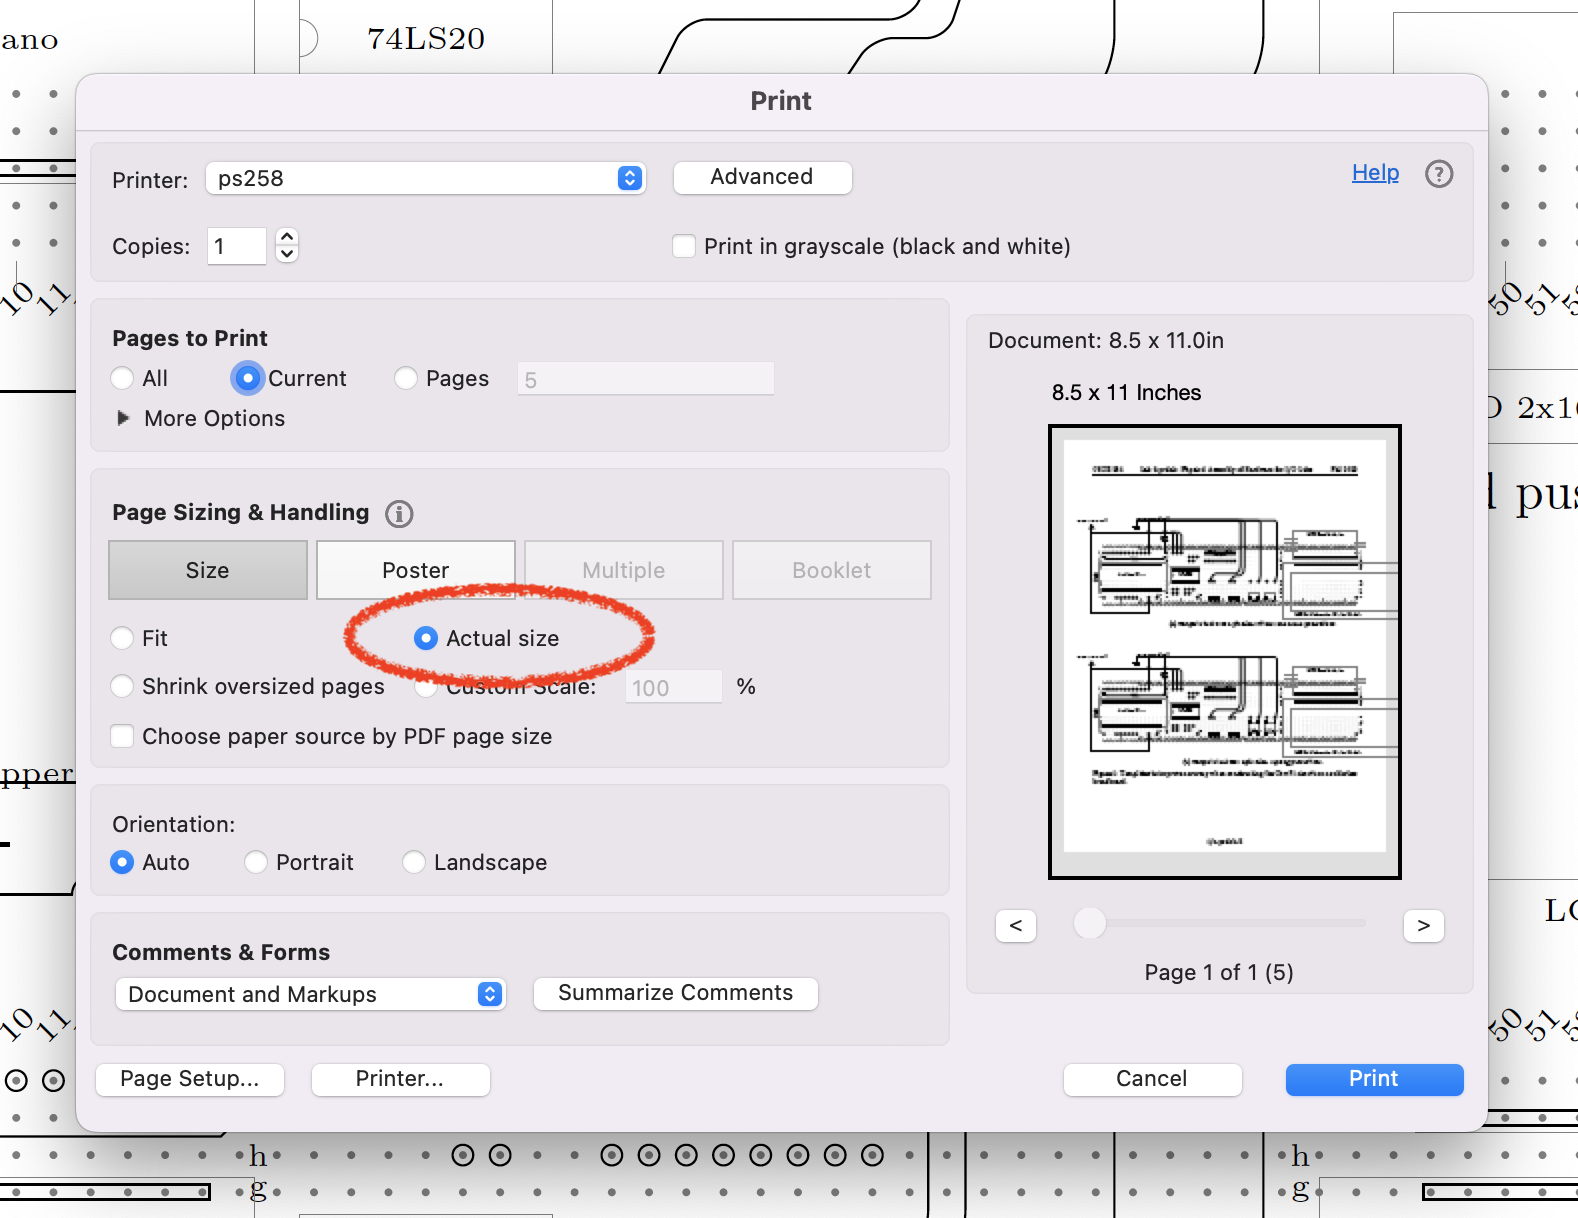
\includegraphics[width=0.5\textwidth]{breadboard-guides/print-menu}
    \caption{When printing a breadboard template, be sure to select ``Actual size''.} \label{fig:printmenu}
\end{figure}

\begin{figure}
    \centering
    \subfloat[Punching alignment holes in breadboard template.]{
        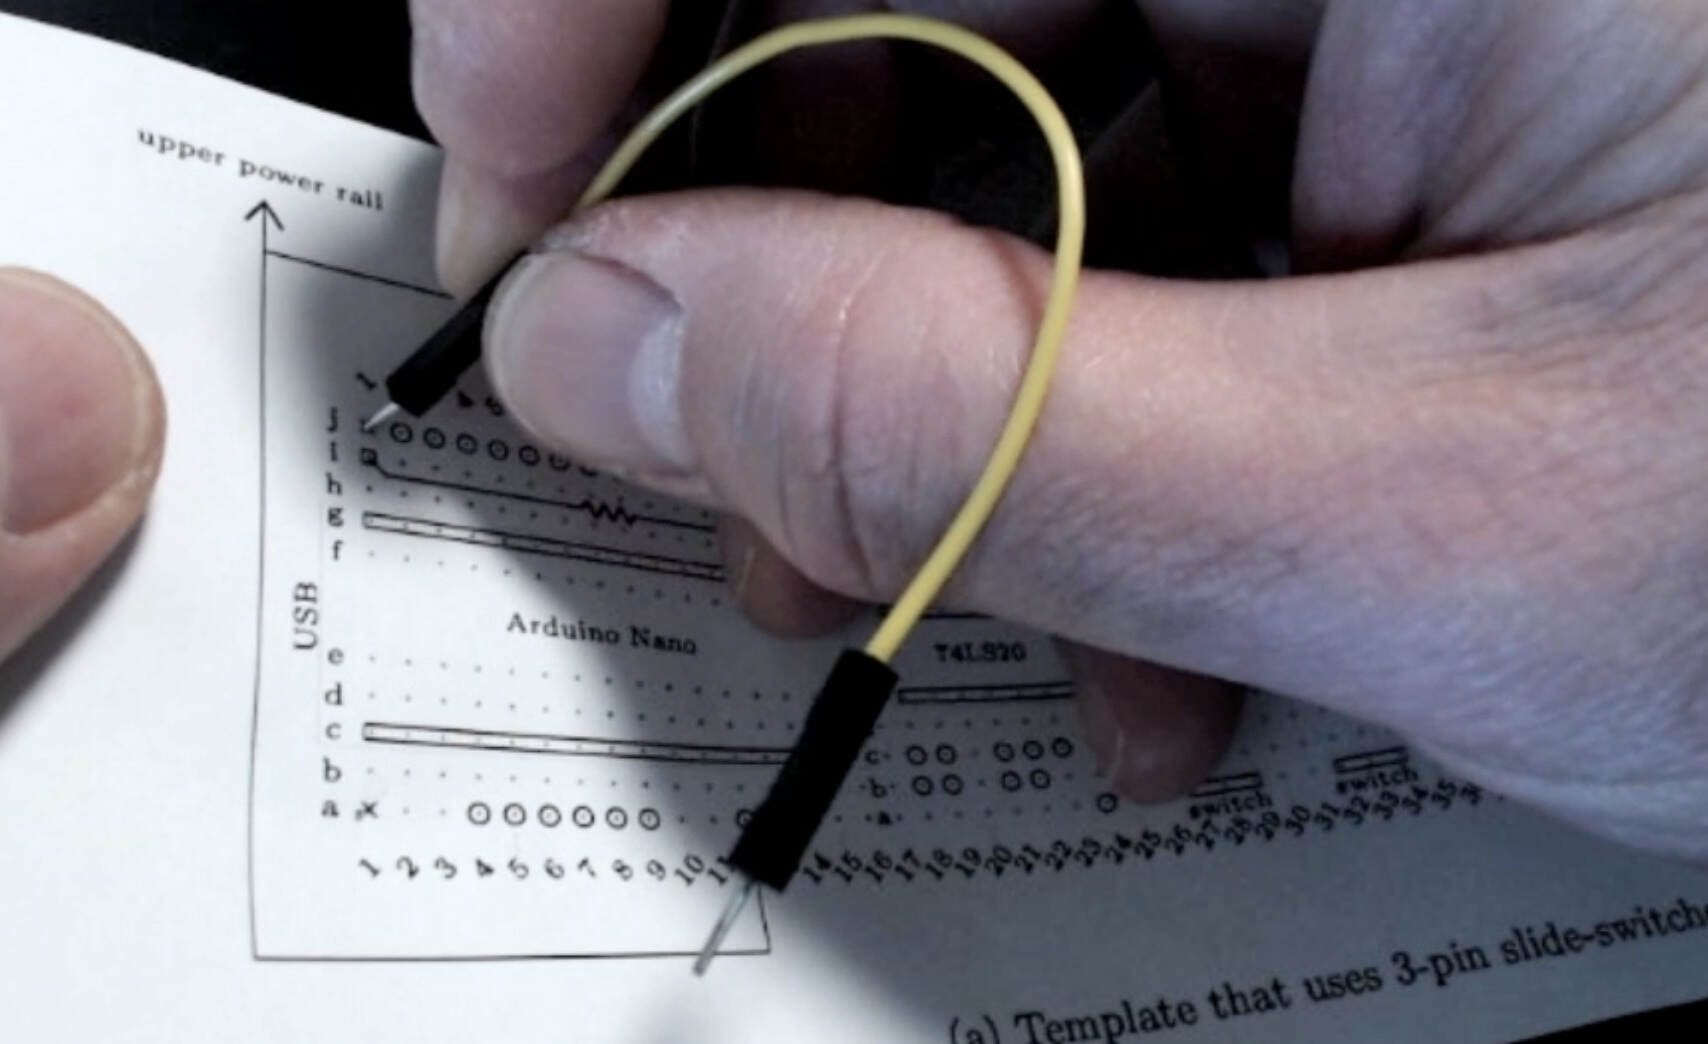
\includegraphics[height=3cm]{breadboard-guides/punching-holes}
        \label{fig:punchingholes}
    }
    \hfil
    \subfloat[Confirming that the corners of the template are aligned with the corners of the breadboard.]{
        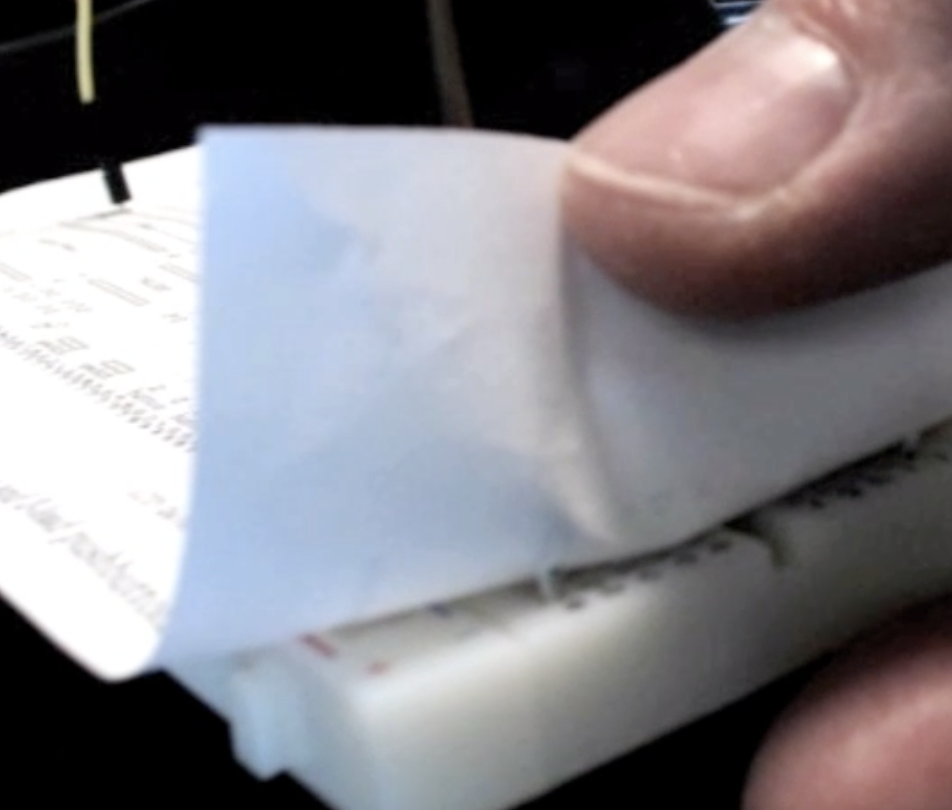
\includegraphics[height=3cm]{breadboard-guides/confirm-alignment}
        \label{fig:confirmalignment}
    }
    \caption{Preparing a breadboard template.}
\end{figure}



%! suppress = MissingImport
\subsection{Install the \developmentboard\ onto the Breadboard}

    \begin{description}
        \checkoffitem{Orient the breadboard in front of you so that row 1 is on your left and row 63 is on your right;
        column a should be at the bottom, and column j should be at the top.}
        \checkoffitem{\prepunch{\mcuupperrow\ and \mculowerrow}
        See Figure~\ref{fig:prepunching}.}
    \end{description}

    After the paper provides some initial resistance, the jumper's lead will slide into the breadboard's contact point;
    remove the lead and move on to the next contact point.
    You want to pre-punch these holes because the paper provides less resistance when you're inserting a single lead than it does when you're inserting a component with multiple leads.

    \begin{figure}
        \centering
        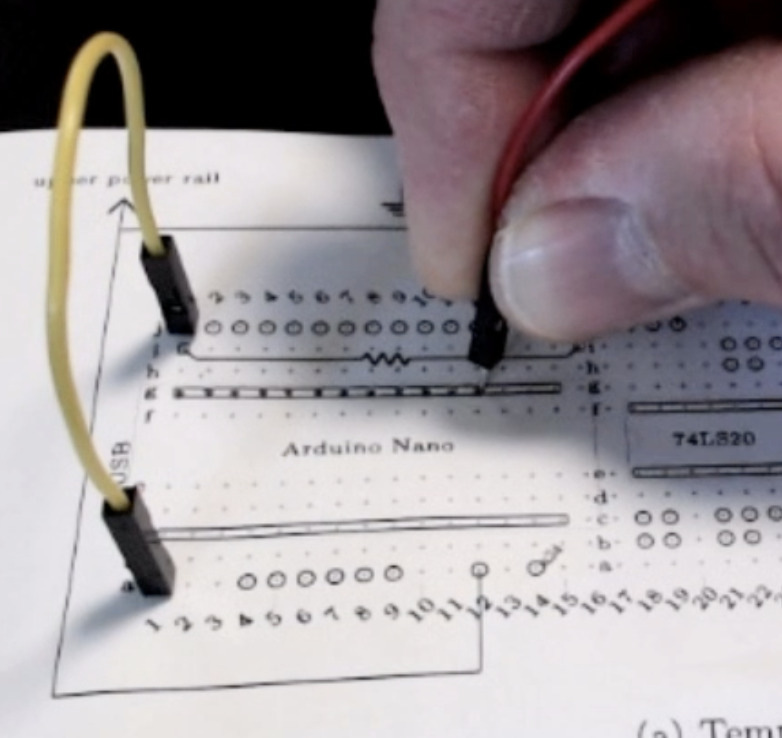
\includegraphics[height=3cm]{microcontroller/breadboard/prepunching}
        \caption{Pre-punching holes in the breadboard template before inserting a component.} \label{fig:prepunching}
    \end{figure}

    \begin{description}
        \checkoffitem{Remove the anti-static foam from the \developmentboard's pins.}
    \end{description}
    You will place the \developmentboard\ on the left side of the breadboard with the USB connector on the left (that is, facing away from the breadboard).
    \begin{description}
        \checkoffitem{Position the upper row of pins on contact points \mcuupperrow\ and the lower row of pins on contact points \mculowerrow.}
    \end{description}
%! suppress = NonMatchingIf
\ifdefstring{\formfactor}{nano}{
    The left side of the \developmentboard\ will obscure the labels for columns c--g.
    The right side of the \developmentboard\ will cover contact points c16--g16 but won't use them.
}{}
\begin{description}
    \checkoffitem{Double-check that:}  % TODO: figure out how to generalize this
        \begin{itemize}
            \item the pin labeled \texttt{D12} is in the upper-left, on contact point g1
            \item the pin labeled \texttt{D13} is in the lower-left, on contact point c1
            \item the pin labeled \texttt{VIN} is in the lower-right, on contact point c15
            \item the pin labeled \texttt{TX1} is in the upper-right, on contact point g15
        \end{itemize}
    \checkoffitem{Gently press on both ends of the \developmentboard\ to insert the pins into the contact points, using a slight rocking motion if necessary (Figure~\ref{fig:inserting-mcu}).}
    \checkoffitem{Press the \developmentboard\ into the breadboard until it physically cannot be inserted any deeper (Figure~\ref{fig:mcu-inserted}).}
\end{description}

%! suppress = NonMatchingIf
\begin{figure}
    \centering
    \subfloat[Press gently on both ends of the \developmentboard.] {
        \ifdefstring{\developmentboard}{Arduino Nano}{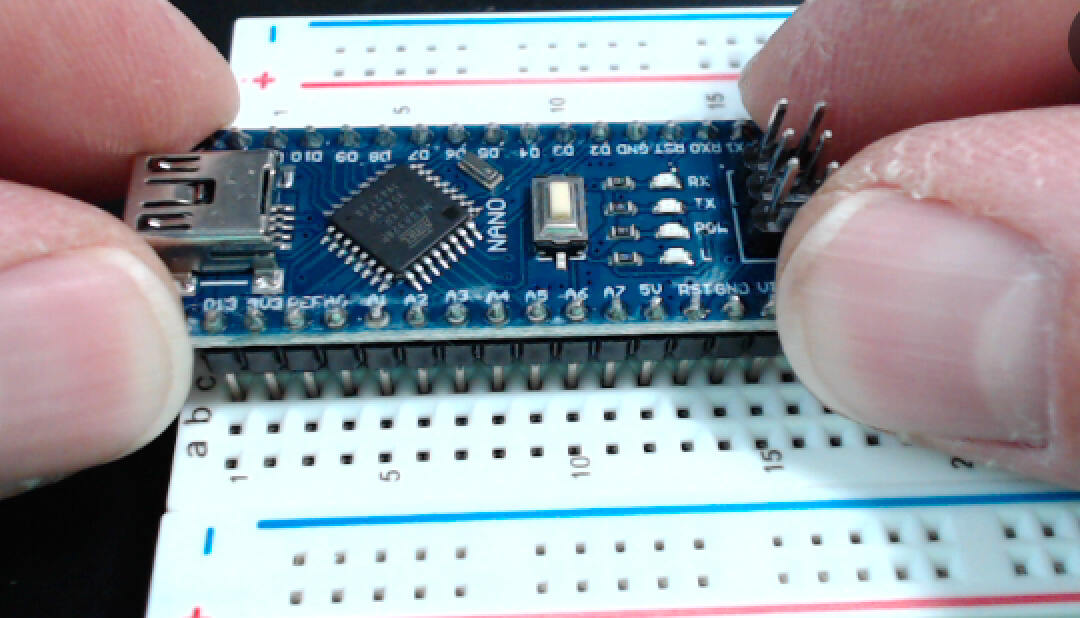
\includegraphics[height=3cm]{microcontroller/breadboard/inserting-nano}}{}
        \label{fig:inserting-mcu}
    }
    \hfil
    \subfloat[The \developmentboard\ fully inserted.] {
        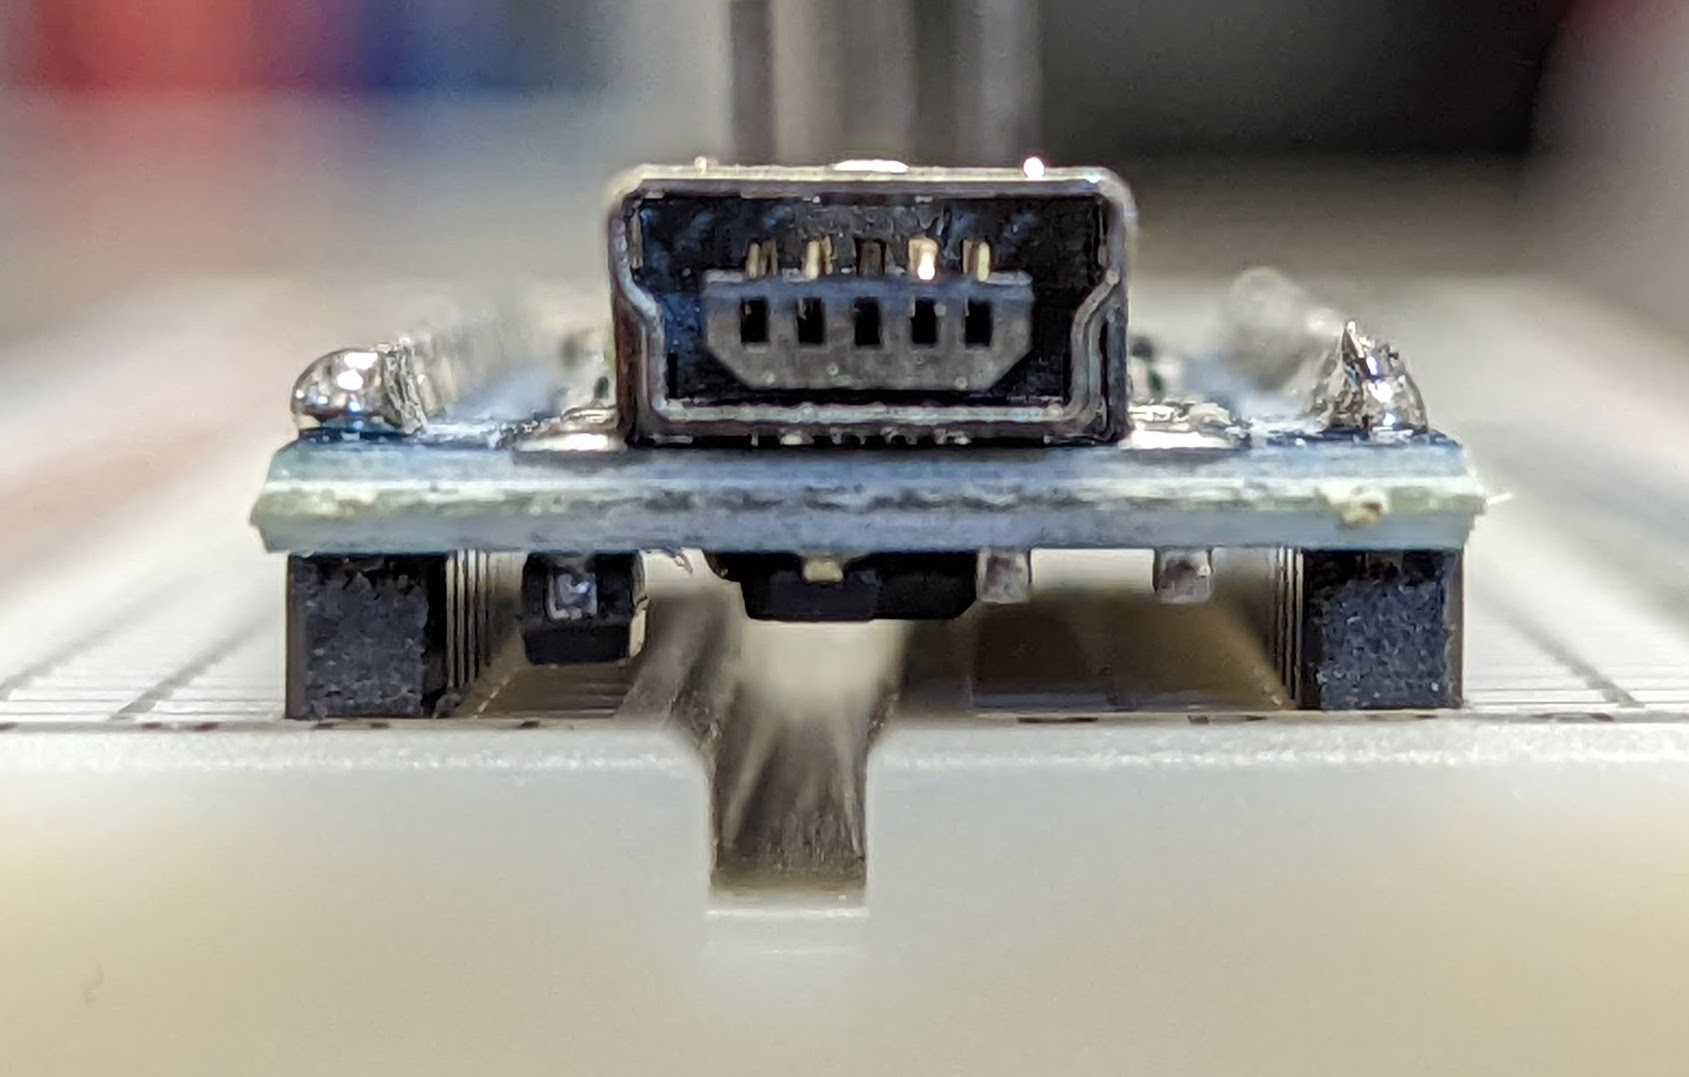
\includegraphics[height=3cm]{microcontroller/breadboard/nano-fully-inserted}
        \label{fig:mcu-inserted}
    }
    \caption{Inserting the \developmentboard\ into the breadboard.}
\end{figure}

\checkpoint{inserted the \developmentboard\ into the breadboard}

\textit{If you are using a breadboard template} then you can now remove the jumper wires from contact points a1 and j1;
the \developmentboard\ will keep the left side of the template pinned in place.


\subsection{Install Arduino IDE}

    The Arduino IDE is installed on the lab computers.
    If you choose to install the Arduino IDE on your personal laptop, you can download it from
    \url{https://www.arduino.cc/en/software}.
    Alternatively, you can install a browser plugin to use the
    \href{https://create.arduino.cc/projecthub/Arduino_Genuino/getting-started-with-arduino-web-editor-on-various-platforms-4b3e4a}{Arduino Web Editor}.
    There are third-party plugins for many other IDEs; however, using these may limit our ability to help you if your have difficulties.

\subsubsection*{About Arduino Programs}

    An Arduino program is called a \textit{sketch} for historical reasons.\footnote{The Arduino language is based off of the Wiring language, which in turn is based off of the Processing language, which was designed to make computing accessible to artists.}
    For all intents and purposes, you can think of it as a C++ program\footnote{Your code in the I/O labs will be C code.} in which you write two functions, \function{setup} and \function{loop}, along with any helper code that you need.
    The file extension for sketches is \textbf{\textit{.ino}} (as in, Ardu\textbf{\textit{ino}}).
    The Arduino IDE will compile your sketch and link it to a \function{main} function that looks something like:
    \begin{lstlisting}
    int main() {
        setup();
        while(true) {
            loop();
        }
    }
    \end{lstlisting}
    (The actual \function{main} function\footnote{\url{https://github.com/arduino/ArduinoCore-avr/blob/master/cores/arduino/main.cpp}} also calls a few other functions from the Arduino core library.)

\subsection{Connect to the \developmentboard}

    \begin{itemize}
        \item Connect one end of the mini-USB cable to a lab computer or to your personal laptop.\footnote{You can connect it to a ``wall wart'' USB power supply to run the \developmentboard, but you need to connect it to a computer to upload a new sketch to the \developmentboard.}
        \item Connect the mini-USB end of the cable to your \developmentboard.
    \end{itemize}
    The \texttt{PWR} LED will light up, and you may see the \texttt{L} LED repeatedly blink on-and-off.
    The \texttt{L} LED is connected to the \developmentboard's pin D13, and Arduino microcontroller boards typically leave the factory with \textit{Blink.ino} loaded, but it does not matter if yours does not have \textit{Blink.ino} pre-loaded.

    \begin{lstlisting}[basicstyle=\ttfamily\footnotesize]
    // the setup function runs once when you press reset or power the board
    void setup() {
      // initialize digital pin LED_BUILTIN as an output.
      pinMode(LED_BUILTIN, OUTPUT);
    }

    // the loop function runs over and over again forever
    void loop() {
      digitalWrite(LED_BUILTIN, HIGH);   // turn the LED on (HIGH is the voltage level)
      delay(1000);                       // wait for a second
      digitalWrite(LED_BUILTIN, LOW);    // turn the LED off by making the voltage LOW
      delay(1000);                       // wait for a second
    }
    \end{lstlisting}

    \begin{description}
        \checkoffitem{Open the Arduino IDE on the computer that your \developmentboard\ is connected to.}
        \checkoffitem{Connect the Arduino IDE to the \developmentboard.}
    \end{description}
    %! suppress = MissingImport
%If you are using Arduino IDE 1.8, see this \href{https://www.arduino.cc/en/Guide/ArduinoNano#select-your-board-type-and-port}{Tutorial} for selecting the \developmentboard\ board, processor, and COM port (or this \href{https://www.arduino.cc/en/Guide/ArduinoUno#select-your-board-type-and-port}{Tutorial for the Arduino Uno}, which has more detail on selecting the COM port).
If you are using Arduino IDE 1.8, see the Quickstart Guide on the \href{https://docs.arduino.cc/hardware/nano}{\developmentboard's documentation page} for selecting the \developmentboard\ board, processor, and COM port.
If you are using Arduino IDE 2.0 or the Arduino Web Editor, COM port should be automatically detected.
You will still need to select the board and processor;
see Figure~\ref{fig:selecting-mcu} and the discussion in Section~\ref{subsubsec:processor-selection}.

\begin{figure}
    \centering
    \subfloat[Selecting the board with Arduino IDE 1.8.] {
        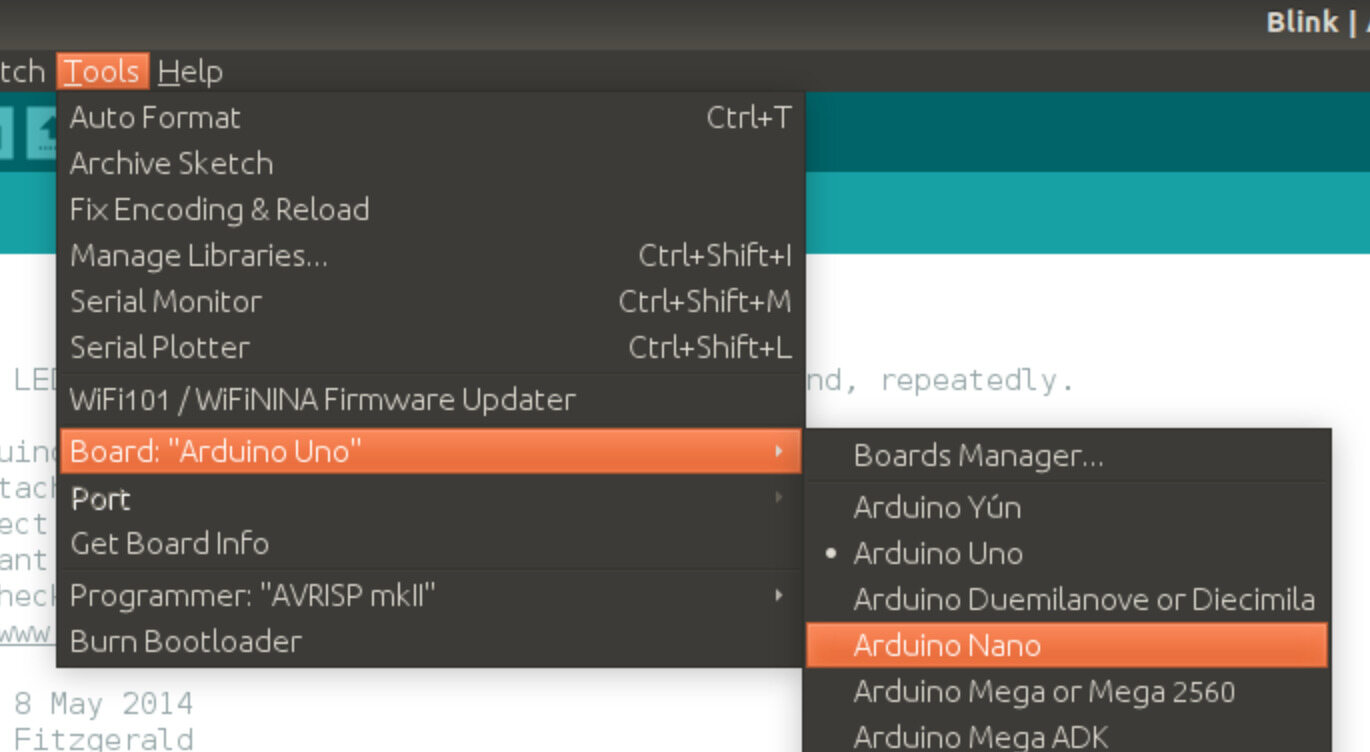
\includegraphics[width=7cm]{microcontroller/ide/selecting-nano-1_8}
%        \label{fig:selecting-board-1}
    }
    \hfil
    \subfloat[Selecting the board with Arduino IDE 2.0.] {
    % 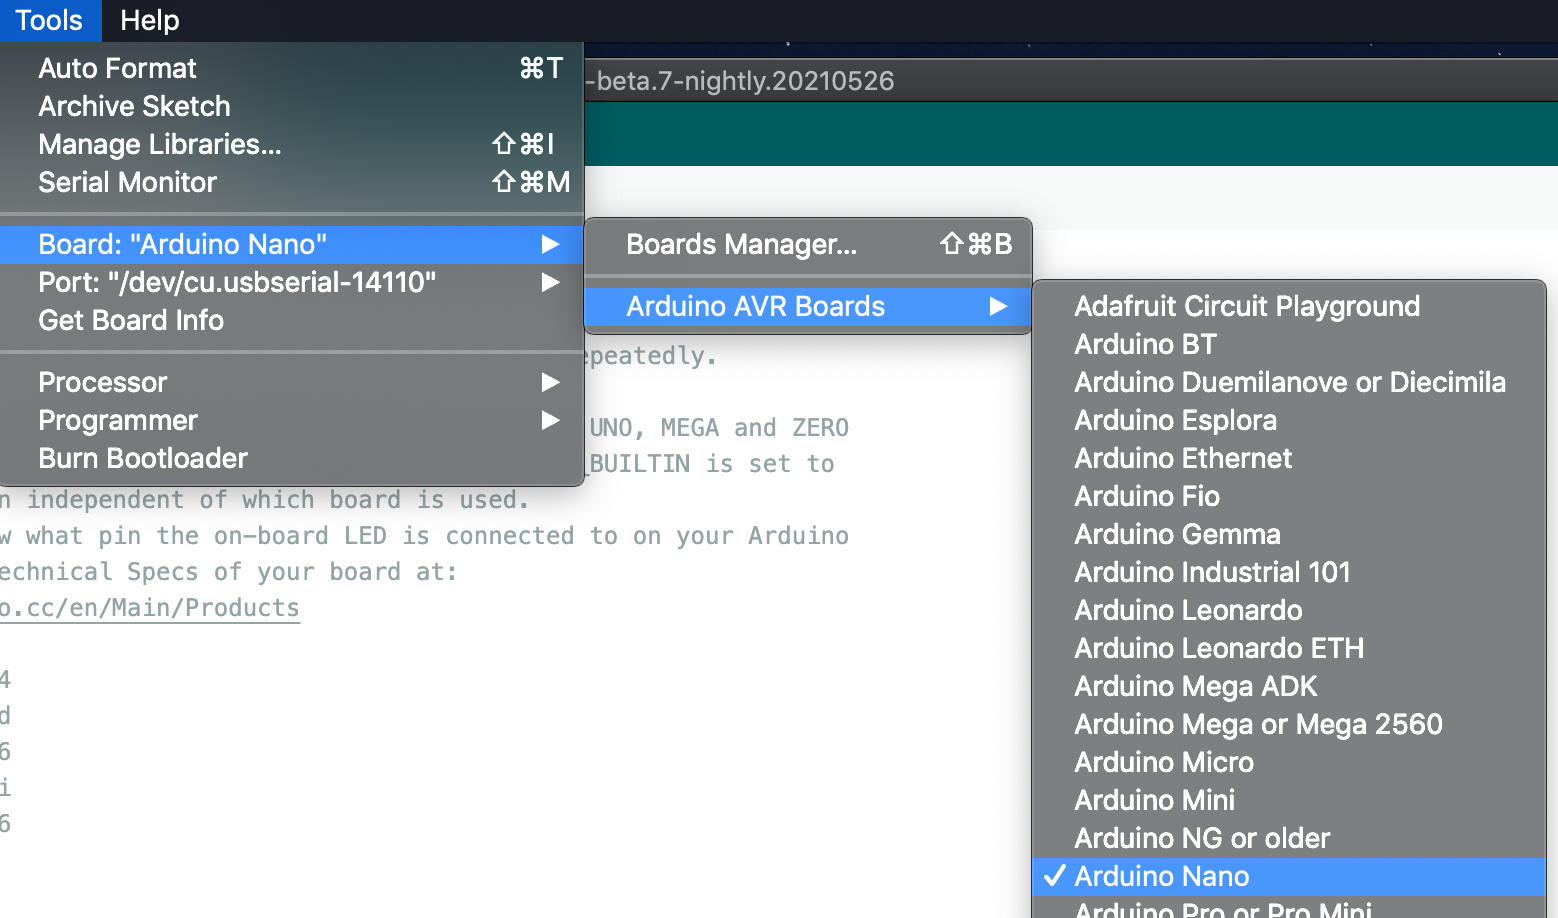
\includegraphics[width=7cm]{selecting-nano-from-menu}
        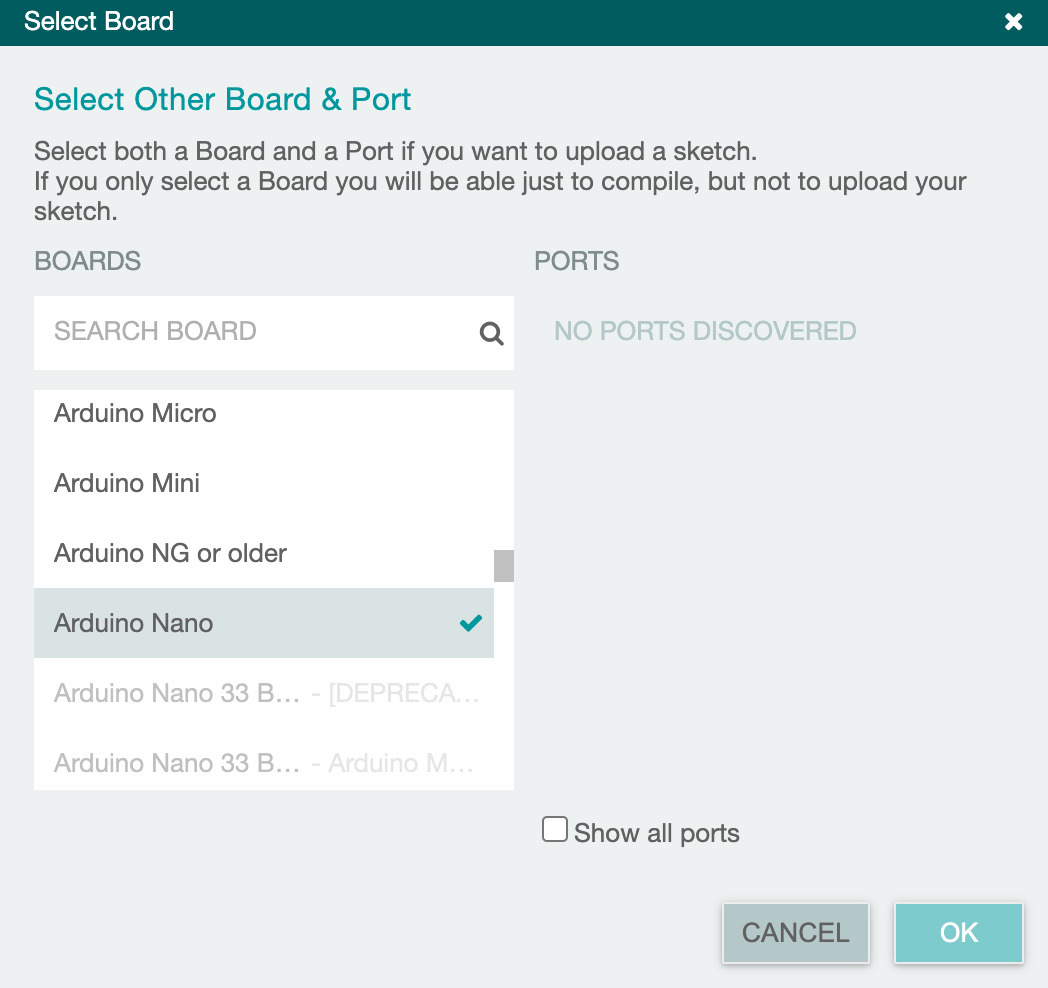
\includegraphics[height=4.1cm]{microcontroller/ide/selecting-nano}
%        \label{fig:selecting-board-2}
    }

    \subfloat[Selecting the processor after selecting the board.] {
    % \vtop{\vskip-4.1cm\hbox{\includegraphics[width=5cm]{selecting-nano-processor}}}
        \includegraphics[width=7cm]{microcontroller/ide/selecting-nano-processor}
        \label{fig:selecting-processor}
    }
    \caption{Selecting board and processor in the Arduino IDE.
    \label{fig:selecting-mcu}}
\end{figure}

\subsubsection{Selecting the Correct ``Processor''}\label{subsubsec:processor-selection}

There are \textit{three} choices for the \developmentboard{}'s processor, two of which specify the ATmega328P processor.
Even though the difference is a USB interface issue, it is resolved through the Arduino IDE's ``Processor'' selection:

\begin{itemize}
    \item Official \developmentboard{}s use the FT232RL USB interface chip.
    Under the ``Tools'' menu, when choosing ``Processor'', select ``ATmega328P''.
    \item \textit{Most} \developmentboard\ clones use the CH340 USB interface chip.
    Under the ``Tools'' menu, when choosing ``Processor'', select ``ATmega328P (Old Bootloader)''.
    (If you are using the Arduino IDE 1.8.4 and earlier, which don't have the ``(Old Bootloader)'' option, simply select ``ATmega328P'').
    \item If you have an older \developmentboard\ that the ATmega168 processor, replace it with one that has an ATmega328P processor.
\end{itemize}

\subsubsection{Updating USB Driver if Necessary}

We have seen some Windows computers without the CH340 USB driver.
If you encounter this problem and the Device Manager shows you the warning in Figure~\ref{fig:usb-warning}, then the first thing to try is updating the driver.
Right-click on USB2.0-Seri! (Figure~\ref{fig:update-driver}) and choose ``Update driver''.
Then choose ``Search automatically for updated driver software''.

\begin{figure}
    \centering
    \subfloat[] {
        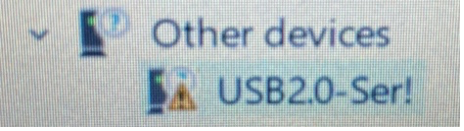
\includegraphics[width=.4\textwidth]{microcontroller/usb-drivers/device-manager-warning}
        \label{fig:usb-warning}
    }
    \hfil
    \subfloat[] {
        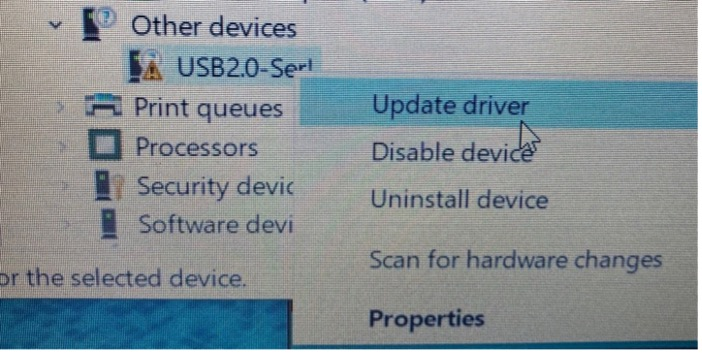
\includegraphics[width=.4\textwidth]{microcontroller/usb-drivers/update-driver}
        \label{fig:update-driver}
    }
    \caption{Selecting board and processor in the Arduino IDE.}
\end{figure}

If Windows reports that ``Windows has successfully updated your drivers'' then you should now be able to connect to the \developmentboard.
On the other hand, if Windows reports that ``Windows was unable to install your USB2.0-Ser!'', then the \href{https://learn.sparkfun.com/tutorials/how-to-install-ch340-drivers/}{How to Install CH340 Drivers} page at sparkfun.com will guide you through manually downloading the driver and installing it.

Sparkfun's \href{https://learn.sparkfun.com/tutorials/how-to-install-ch340-drivers/}{How to Install CH340 Drivers} page also has instructions for installing the driver on MacOS and on Linux;
however, we are not aware of any students needing to manually install the CH340 driver on MacOS\@.

\subsubsection{No Driver Warning but Cannot Connect}

Probably what happened is that your computer has the driver, but you're telling the IDE to connect to the wrong virtual COM port.
The typical way to handle this is to disconnect the \developmentboard\ from your computer, go to the part of the menu where you connect to the COM port, connect the \developmentboard\ to your computer, and select whichever COM port appears after plugging in the \developmentboard.


\subsection{Upload a New Sketch}

    \begin{description}
        \checkoffitem{From the Arduino IDE's File menu, open the \textit{Blink.ino} example:} \\
            \textit{File} $\rightarrow$ \textit{Examples} $\rightarrow$ \textit{01.Basics} $\rightarrow$ \textit{Blink} \\
            Select \textit{Save As...} and save the project as \textit{MyBlink}.
        \checkoffitem{Edit the values in the \function{delay} calls to change the delays between the LED turning on, off, and on again.
        Select values that will visibly have a difference, such as 250 or 2000.}
        \checkoffitem{Compile the program using the ``Verify'' checkmark in the IDE's toolbar and make corrections if the program doesn't compile.}
        \checkoffitem{Upload the program to your \developmentboard\ using the ``Upload'' arrow in the IDE's toolbar.
            (If you forget to compile first, the IDE will compile your program before uploading, but I find it useful to find compile-time mistakes before attempting to upload the program.)}
    \end{description}

    If you successfully uploaded \textit{MyBlink.ino} then you will see the following in the IDE's \textit{Output} window:
    \begin{quote}
    \dots (elided configuration data)\dots
    \begin{verbatim}
    avrdude: AVR device initialized and ready to accept instructions

    Reading | ################################################## | 100% 0.01s

    avrdude: Device signature = 0x1e950f (probably m328p)
    avrdude: reading input file "/var/folders/p7/lx4gt70d0_34cpy8r0j3c95c0000gp/T/arduino-sketch-11A4823C54657006C9F78B0812B621A8/MyBlink.ino.hex"
    avrdude: writing flash (932 bytes):

    Writing | ################################################## | 100% 0.33s

    avrdude: 932 bytes of flash written

    avrdude done.  Thank you.


    --------------------------
    upload complete.
    \end{verbatim}\end{quote}
    and then the LED's on-off pattern will change, reflecting the \function{delay} values you assigned (Figure~\ref{fig:myblink}).

    \subsubsection*{Handling Errors}

        If you get an error when attempting to upload a sketch, try these corrective measures:

        \begin{enumerate}
            \item Try selecting ``ATmega328P'' and try selecting ``ATmega328P (Old Bootloader)'' (see Figure~\ref{fig:selecting-processor}).
            \item Try uploading again (if you attempt to upload a sketch too soon after connecting your \developmentboard\ to your computer, the USB interface won't have finished its handshake).
            \item The \href{https://support.arduino.cc/hc/en-us/articles/4401874331410--Error-avrdude-when-uploading}{Troubleshooting Guide} recommends disconnecting your \developmentboard\ and reconnecting it, then selecting whichever COM port appears.
        \end{enumerate}

        If, instead of an error, your IDE ``hangs'' while collecting configuration data, try this corrective measure:

        \begin{itemize}
            \item Press the \texttt{RESET} button in the middle of the \developmentboard; the IDE should begin uploading the sketch after you release the button.
        \end{itemize}

    \begin{figure}
        \centering
        \animategraphics[autoplay,loop,height=4cm]{8}{microcontroller/animations/myblink-}{0}{6}
        \caption{\textit{MyBlink.ino} has a different on-off pattern than \textit{Blink.ino}.\label{fig:myblink}}
    \end{figure}

\checkpoint{uploaded new code to the \developmentboard}
